%======================================================================
\subsection{MOD-03 plan: configurations (25 Oct 2026)}\label{sec:mod03-plan}
%======================================================================

\eref{MOD-03} lets one part or assembly file hold several variants: a bracket in three lengths, a gearbox
with and without its encoder. Fusion calls them configurations (a table of rows over parameters, feature
suppression and properties); SolidWorks has configurations and design tables, and each configuration can
carry its own part number. This chapter was written on 25 Oct and building started the same evening, on
your instruction to build on my recommendations; decisions are marked \emph{Decided} with the reason, and
the open ones are in section~9.

%----------------------------------------------------------------------
\subsubsection*{1. What FreeCAD 1.1 already has}

The first version of this roadmap said FreeCAD has no configuration table. That was wrong: Spreadsheet has one
(right-click a sheet, \emph{Configuration Table\dots}, \file{src/Mod/Spreadsheet/Gui/DlgSheetConf.cpp}).
It adds a dynamic \code{PropertyEnumeration} to an object, takes its items from a column of names, and
\emph{binds} one sheet row to the row of the chosen name, so every alias on that row reads the active
configuration's value. \code{App::Link} completes it: an enumeration marked \code{CopyOnChange} shows up
on every link to the object, and choosing another value there copies the linked object (and what it depends
on) into the link's document with that value (\code{LinkCopyOnChange}: \emph{Enabled}, \emph{Owned},
\emph{Tracking}; \file{src/App/Link.cpp}). So stock FreeCAD can already show a Short and a Long bracket side
by side in one assembly. What it lacks: a table you can read (it is a raw sheet with hidden bindings),
suppression and part numbers per row, a way to pick a configuration that does not depend on the part's own
active row, the BOM and the vault.

Measured headless on a bracket (Pad length and a boss's suppression bound to the table, P/N bound to it too):
switching rows gives lengths 50 / 80 / 120\,mm and P/Ns \code{-S/-M/-L}; four links with \emph{Tracking}
show their own rows; a value changed in the part file reaches the copies at the next recompute; the
assembly saves and reopens with every link still in its row.

%----------------------------------------------------------------------
\subsubsection*{2. Data model}

\textbf{Decided:} configurations are FreeCAD's own configuration table, not the \code{FeaturePython}
\code{ConfigurationTable} this roadmap first proposed. \emph{Reason:} a file must open in stock FreeCAD 1.1;
there the native table still switches (property editor) and links still pick rows, while a Python object
would load as a dead placeholder. Link \code{CopyOnChange} also needs a real enumeration on the linked object.

\begin{itemize}
  \item \textbf{The switch.} A \code{PropertyEnumeration} named \code{Configuration} (group
        \emph{Configuration}, status \code{CopyOnChange}) on the file's \emph{main object}: the
        \code{App::Part} that carries the part properties, the \code{Assembly}, or a lone \code{Body}
        (\code{freecad\_io.main\_object}, the object the vault numbers). Assemblies link to it, so links see it.
  \item \textbf{The table.} A spreadsheet \code{Configurations} at the root of the file, laid out so it reads
        well in stock FreeCAD (Figure~\ref{fig:mod03-table}): row~1 the file's own P/N
        (\code{FilePartNumber}); row~2 headers; row~3 the \emph{active} row, bound to the selected row, whose
        aliases the model reads; rows 4\dots\ one per configuration, the name in column A.
  \item \textbf{Columns}, known by the alias on row~3:
        \code{PartNumber} and \code{Description} (bound to the main object's properties); a parameter name
        (a configured parameter); \code{sup\_<Feature>} (0/1, bound to the feature's \code{Suppressed});
        \code{cfg\_<Link>} (assemblies: which configuration that instance uses).
\end{itemize}

\begin{figure}[ht]
\centering
\small
\begin{tabular}{@{}r|l|l|l|l|l@{}}
\multicolumn{1}{c}{} & \multicolumn{1}{c}{A} & \multicolumn{1}{c}{B} & \multicolumn{1}{c}{C} &
  \multicolumn{1}{c}{D} & \multicolumn{1}{c}{E}\\\hline
1 & File P/N & \code{BW-1001} & & & \\\hline
2 & \textit{Configuration} & \textit{length} & \textit{P/N} & \textit{Description} & \textit{Suppress Boss}\\\hline
\textcolor{bwblue}{3} & \textcolor{bwblue}{\code{=Part.Configuration}} & \textcolor{bwblue}{80} & \textcolor{bwblue}{BW-1001-M} & \textcolor{bwblue}{Bracket 80} & \textcolor{bwblue}{1}\\
  & & \textcolor{bwblue}{\code{length}} & \textcolor{bwblue}{\code{PartNumber}} & \textcolor{bwblue}{\code{Description}} & \textcolor{bwblue}{\code{sup\_Boss}}\\\hline
4 & Short & 50 & BW-1001-S & Bracket 50 & 0\\\hline
5 & Standard & 80 & BW-1001-M & Bracket 80 & 1\\\hline
6 & Long & 120 & \code{=FilePartNumber} & Bracket 120 & 0\\\hline
\end{tabular}

\smallskip
\begin{minipage}{0.92\linewidth}\raggedright\footnotesize
Row 3 (blue, with its aliases under it) is bound to the active row: \code{Part.Configuration} lists
column A from row 4 down and grows with it. The model reads row 3:
\code{Parameters.length} $\leftarrow$ \code{=Configurations.length},\;
\code{Pad.Length} $\leftarrow$ \code{Parameters.length},\;
\code{Boss.Suppressed} $\leftarrow$ \code{Configurations.sup\_Boss},\;
\code{Part.PartNumber} $\leftarrow$ \code{Configurations.PartNumber}.
\end{minipage}
\caption{The \code{Configurations} sheet of a bracket with three configurations. Long has no P/N of its own
(\code{=FilePartNumber}), so it is the file's item; Short and Standard are vault items of their own.}
\label{fig:mod03-table}
\end{figure}

\paragraph{Theory.} With parameters $\mathbf p$ and suppression $\mathbf s\in\{0,1\}^F$, configuration $j$
is the row $c_j=(\mathbf p_j,\mathbf s_j,\pi_j)$ and the model is $M(\mathbf p_j,\mathbf s_j)$. The binding
makes the active row a function $r(e)$ of the enumeration index $e$, $r(e)=e+4$, so a switch is one property
write and one recompute; nothing is copied inside the part file. A link with its own configuration holds a
copy $M(\mathbf p_k,\mathbf s_k)$ in the assembly file, so an assembly that uses $m$ distinct configurations
of a part holds at most $m$ copies when links of the same row share one (section~9, question~2); today each
configured link has its own, and a link array shares one for all its elements.

\paragraph{Parameters.} \textbf{Decided:} configuring a user parameter keeps its row in the Parameters sheet
(\eref{MOD-02}) and turns its cell into \code{=Configurations.<name>}; configuring a model dimension that is
not a parameter binds the feature property to the table directly (\code{<Feature>\_<Property>}).
\emph{Reason:} the Parameters tab stays the one place that shows every value, and features that already read
\code{Parameters.length} need no change. A parameter that lives in another file's sheet (the product sheet of
\eref{MOD-02}) is refused, with the reason: a part's configurations change only its own file.

\paragraph{Suppression.} \textbf{Decided:} a \code{sup\_} column binds the feature's \code{Suppressed}
(PartDesign features and Assembly joints have it in 1.1). Components have no suppression in 1.1, so in an
assembly a \code{sup\_<Link>} column binds a BruceWorx \code{Suppressed} property on the link; a suppressed
component is hidden, left out of the BOM, and its joints are suppressed with it when the row is applied.
In stock FreeCAD only the hiding and the joints do not follow.

%----------------------------------------------------------------------
\subsubsection*{3. Picking a configuration in an assembly}

\textbf{Decided:} an instance uses FreeCAD's \code{LinkCopyOnChange = Tracking}, and choosing a configuration
always makes the instance's own copy, even when the row equals the part file's active one. \emph{Reason:} a
link without a copy follows the part's \code{Configuration} (FreeCAD syncs it), so switching the part file
would silently change every assembly that uses it; with a copy each instance says which row it uses, as in
SolidWorks. \emph{Tracking} re-copies when the part file changes, so edits still arrive. A link nobody gave a
configuration (stock \emph{Insert}) shows the file's active row and the Properties tab says ``follows the
part''.

In an assembly's own table, a \code{cfg\_<Link>} column drives an instance's configuration by expression, so
\emph{Gearbox--Short} can use the Short bracket.

%----------------------------------------------------------------------
\subsubsection*{4. Part numbers, the vault and the BOM}

\textbf{Decided:} a configuration with its own P/N is a vault item of its own, a \emph{configuration item}
(\code{configuration\_of} the file's item, and the row name). It has no file: it shares the file item's
revisions and state, because one file has one revision, as SolidWorks PDM does it. Lifecycle steps on it are
refused with ``change \emph{BW-1001}, its file''; retiring the file's item retires its configurations.
A row with no P/N of its own (\code{=FilePartNumber}) is the file's item.
\begin{itemize}
  \item \textbf{Numbers.} Typed in the P/N column, or \emph{Assign Number} from the vault's numbering
        (the next number in the file's program).
  \item \textbf{Check-in} reads the table and adds configuration items that are missing (description from
        the row); a P/N that already names another item is refused before the file is stored.
  \item \textbf{BOM} (\eref{PDM-06}, \file{bruceworx\_bom.py}): the walker follows a link's copy back to its
        part file and offers the copy's own P/N first, so three brackets in three rows are three lines and two
        Long ones are one line with quantity~2.
  \item \textbf{Open from Vault} on a configuration item opens the file in that configuration.
\end{itemize}

%----------------------------------------------------------------------
\subsubsection*{5. UI}

\begin{itemize}
  \item \textbf{Parameters tab} (\eref{UIX-12}): a configuration bar on top when the file has
        configurations, with the active row in a drop-down (switch and recompute, one undo step) and
        \emph{Table\dots}; a configured parameter shows its row value and a small ``per configuration'' mark.
  \item \textbf{Configuration Table} (Modify \textrightarrow{} \emph{Configurations\dots}, also from the
        bar): rows are configurations, columns P/N, Description, then parameters and suppressions. Add,
        duplicate, rename and delete rows; \emph{+ Column} for a parameter, a model dimension, a feature's
        suppression or (assemblies) an instance's configuration; \emph{Check All} (below); CSV export and
        import, as with a SolidWorks design table. Edits go into the sheet as one undo step.
  \item \textbf{Instances}: the Properties tab of a selected link to a configured part shows a
        \emph{Configuration} drop-down; the Browser shows the row after the name (\emph{Bracket
        $\cdot$ Long}).
\end{itemize}

\textbf{Decided: Check All.} Applies each row in turn, recomputes, and lists the features that fail in
which rows, then restores the active one. \emph{Reason:} the topological-naming risk in the roadmap
(a fillet on an edge that only exists when another feature is on) shows up only in the rows that are not
active.

%----------------------------------------------------------------------
\subsubsection*{6. Stock FreeCAD}

Everything in the file is a native object: a sheet, an enumeration, expressions and links. In FreeCAD 1.1.4
the part opens in its saved row, the \code{Configuration} property switches it, and an assembly's links keep
their rows. Lost in stock: the table dialog, component hiding when suppressed, and the vault.

%----------------------------------------------------------------------
\subsubsection*{7. Acceptance test}

A bracket with three configurations, Short / Standard / Long (50 / 80 / 120\,mm, the boss suppressed in
Short), two of them with their own vault numbers. An assembly holds one Short, one Standard and two Long.
On a copy of the vault: check-in adds the configuration items; the assembly's BOM has three lines with the
right P/Ns and quantities 1, 1, 2; \emph{Check All} is clean; both files open in stock FreeCAD 1.1.4 with
the same shapes.

%----------------------------------------------------------------------
\subsubsection*{8. As built (25 Oct)}

Built as planned in four commits, then one fix the acceptance run found. Code (in
\file{src/Mod/BruceWorx/}): \file{bruceworx\_configs.py} (engine, no GUI),
\file{bruceworx\_configs\_gui.py} (table window, Parameters bar, drop-downs, vault hook),
small hooks in \file{bruceworx\_parameters.py}, \file{bruceworx\_inspector.py},
\file{bruceworx\_bom.py} and \file{bruceworx\_vaultclient.py}; in the vault engine
\code{Vault.add\_configuration} (journal op, contract row T14, OpenAPI path) and
\code{freecad\_io.set\_part\_number}.

\begin{figure}[ht]
\centering
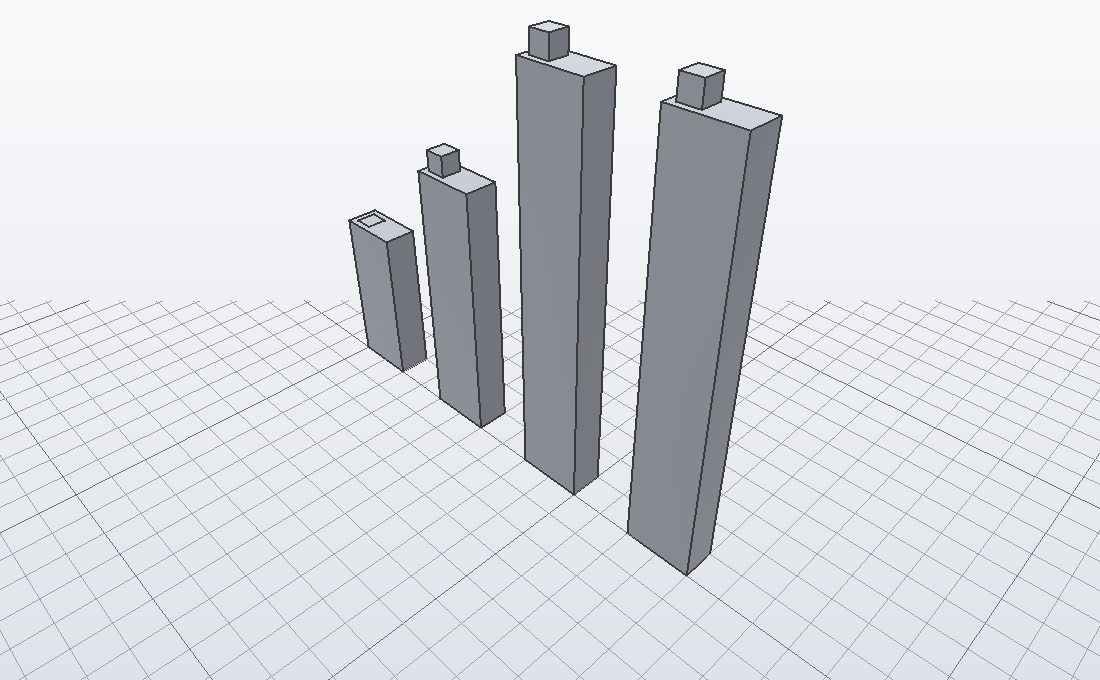
\includegraphics[width=0.49\linewidth]{fig/mod03_frame.png}\hfill
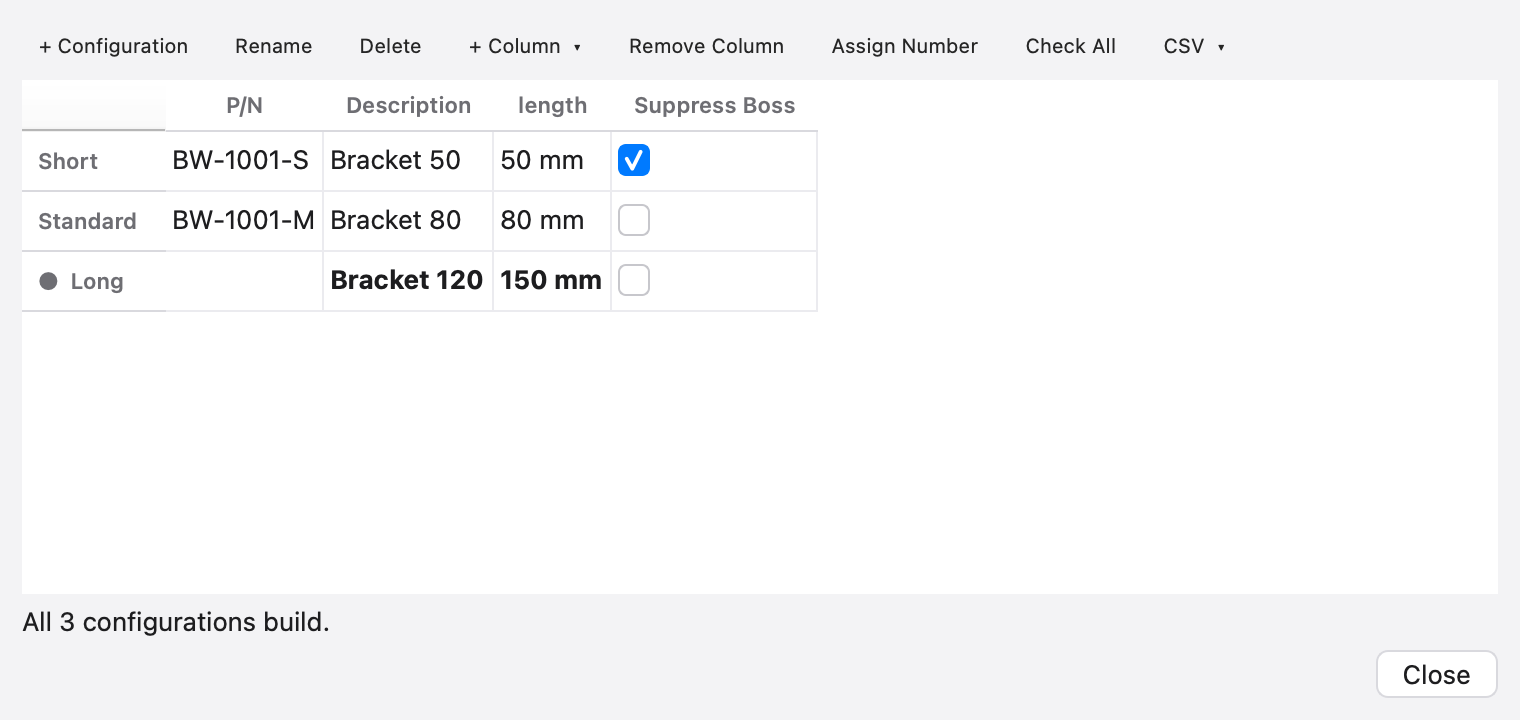
\includegraphics[width=0.49\linewidth]{fig/mod03_table.png}\\[4pt]
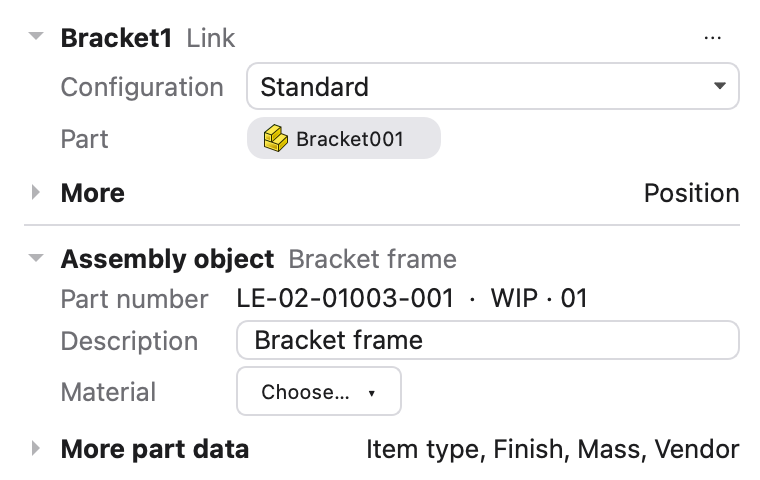
\includegraphics[width=0.40\linewidth]{fig/mod03_inspector.png}
\caption{The acceptance run on a copy of the Vector vault. Left: the frame \code{LE-02-01003-001} with one
Short (boss suppressed), one Standard and two Long instances of the one bracket file
\code{LE-01-01017-001}. Right: its Configuration Table (Long has no number of its own, so it shows the
file's P/N in grey italic). Below: the Properties tab of an instance, with its Configuration drop-down.}
\label{fig:mod03-built}
\end{figure}

\paragraph{Decided while building.}
\begin{itemize}
  \item \textbf{Configuration numbers are dash numbers.} \emph{Assign Number} takes the next sub-number under
        the file's parent drawing (\code{LE-01-01017-001} $\rightarrow$ \code{-002}, \code{-003}), reserved in
        the vault's numbering. \emph{Reason:} the family reads as one in the vault and on drawings, the way
        SolidWorks tabulated drawings use \code{-001}, \code{-002}.
  \item \textbf{Configuration items have their own revision views.} They show the file item's revisions
        (same code, state and history) through a view per revision, because the BOM graph keys revisions by
        identity and two items sharing one object merged their quantities. A configuration item cannot be
        checked out or in; its versions are the file's.
  \item \textbf{Copies are never the assembly's own.} An instance's copy brings the part's
        \code{Configurations} and \code{Parameters} sheets into the assembly; the table, the main object,
        the Parameters tab and the model parameter list skip anything in a \code{CopyOnChangeGroup}, and
        expressions name the assembly's own sheet by its object name (\code{Configurations001} when a copy
        took the name first).
  \item \textbf{An empty text cell is \code{=<<>>}.} A lone quote leaves the cell without a value, and an
        alias on it fails (an assembly without a P/N had a broken table until this).
  \item \textbf{Settle the copies.} When the part changes, FreeCAD (stock 1.1.4 too) copies a
        \emph{Tracking} instance again and shows the part's active row until the next recompute;
        \code{settle\_copies} recomputes while a copy is left touched (after a switch, after picking a row,
        after every recompute, before the BOM walk). In stock FreeCAD a second recompute does the same.
\end{itemize}

\paragraph{Tests and results.}
\begin{itemize}
  \item \code{TestBruceWorxConfigs} (FreeCADCmd, 18 tests): table layout and the native binding, switching
        (heights 50 / 86 / 126\,mm, P/Ns per row, boss suppressed in Short), parameter, dimension,
        suppression and instance columns coming and going, rows added, renamed and removed, Check All
        finding a pad of length 0 in one row, CSV round trip, save and reopen, four instances keeping
        their rows across a part change and a reopen, an assembly table driving an instance, component
        suppression (hidden, joint off, not a BOM line), dash numbers and configuration items in a scratch
        vault, the BOM walk (one line per configuration).
  \item Vault engine: 470 tests pass, with T14 run against the model and the folder vault and a replay test.
  \item GUI: the Parameters bar lists and switches the rows (one undo step each), the table edits a length
        and a suppression, Check All reports ``All 3 configurations build'', and the instance drop-down sets
        rows.
  \item \textbf{Acceptance} (GUI, vault copy): New Part in Vault, three rows, \emph{Assign Number} twice,
        check-in added configuration items \code{-002} (Short) and \code{-003} (Standard); the frame's
        check-in recorded the BOM \code{-002}\,$\times$1, \code{-003}\,$\times$1, \code{-001}\,$\times$2 with no
        missing lines; Check All clean; \emph{Open from Vault} on \code{-002} opened the bracket in Short.
        Volumes 10\,000 / 16\,216 / 24\,216\,mm$^3$.
  \item \textbf{Stock FreeCAD 1.1.4} (\file{/Applications/FreeCAD.app}): both files open with no invalid
        objects; the four instances show Short, Standard, Long, Long with their P/Ns; the part's
        \code{Configuration} property switches it with the same volumes and P/Ns.
\end{itemize}

\paragraph{Not built yet.} The Browser does not show an instance's row after its name (the Properties tab
does); the Properties tab names an instance's part by its copy's label (\emph{Bracket001}); a configured
parameter in the Parameters tab shows its expression \code{Configurations.length} rather than a
``per configuration'' mark (its value edits go to the active row).

%----------------------------------------------------------------------
\subsubsection*{9. Build order and questions}

Pieces, each tested and committed: (1) this plan; (2) the engine \file{bruceworx\_configs.py} (table,
rows, columns, apply, Check All, instances), tested headless; (3) BOM keys and configuration items in the
vault; (4) the Parameters bar, the table dialog and the instance drop-down; (5) the acceptance test, in the
GUI and in stock FreeCAD.

\begin{enumerate}
  \item \textbf{Configuration items share the file's revision.} Releasing the file releases every
        configuration in it; one cannot be released alone. That is SolidWorks PDM's way.
        \emph{Recommendation:} keep it. The other choice, a revision per configuration, means files whose
        rows are in different states.
  \item \textbf{One copy per instance.} Each configured link copies the part's feature tree into the
        assembly file (a bracket adds about 25 objects). Links of the same row could share one hidden
        holder; it changes how joints address the part. \emph{Recommendation:} keep one copy each until an
        assembly is slow; link arrays already share.
  \item \textbf{Vault BOM of a configured assembly.} An assembly with configurations records the BOM of the
        row it was saved in; its configuration items share that BOM. \emph{Recommendation:} a BOM per
        configuration item next, after you have used this on a real assembly.
  \item \textbf{Drawings.} A drawing view of a configured part shows the part's active row. Should a view
        pick its own row (SolidWorks does)? \emph{Recommendation:} yes, with \eref{DRW-01}'s next pass, through
        the same link copy.
\end{enumerate}
